%Name: Template of COMP9020 Assignments
%Author:Jack
%Date: 14/08/2017
%Acknowledgement: This template is based on work of Brendan Trinh of UNSW MathSoc 2015
\documentclass[11pt, a4paper]{article}

\usepackage{amsmath} % Improves structure of typed out maths
\usepackage{mathtools} % Improves upon deficiencies of amsmath package
\usepackage{amssymb} % Adds some handy symbols to use.
\usepackage{amsthm} % Adds some neat formulas to use, e.g. \begin{proof} etc.

\usepackage[a4paper]{geometry} % Default page margins can be altered.
\usepackage{microtype} % Improves spacing between letters.
\usepackage{booktabs} % Improves tables. Can now create without vertical separators.
\usepackage{array} % Includes more options for arrays
\usepackage{paralist} % More flexible use of itemize, enumerate, etc.
\usepackage{graphicx} % Add images to your document
\usepackage{color} % Allows for the use of colours!
\usepackage{cleveref} % Better cross-referencing
\usepackage{hyperref} % For adding hyperlinks
\usepackage{fancyhdr} % Customise headers & footers in document
\usepackage{paralist}

\usepackage{url} % For adding url

\begin{document}
\title{COMP9311 - Assignment 3}
\author{Jack Jiang (z5129432)}
\date{ 8 October 2017 }
\maketitle
\graphicspath{{/}}


\section*{Question 1}
\renewcommand{\labelenumi}{\roman{enumi}. }
\begin{enumerate}
    \item    
        \begin{enumerate}
            \item 
                Since we don't have EF, so every candidate keys must include E and F
                ACEF
                BCEF
            \item
                Key = ACEF, AD $\to$ B violate BCNF
            \item 
                \{ABCDEF\} FD = \{AD$\to$B, C$\to$D, BC$\to$A, B$\to$D \} KEY = ACEF\\
                to fix AD$\to$B, decompose into: \{ABD\}\{ACDEF\}\\
                \{ABD\} FD = \{AD$\to$B, B$\to$D\} KEY = AD\\
                to fix B$\to$D, decompose into: \{BD\}\{AB\}\\
                \{ACDEF\} FD = \{C$\to$D\} KEY = ACEF\\
                to fix C$\to$D, decompose into: \{ACEF\}\{CD\}\\
                Therefore, the collection of BCNF is \{AB, BD, CD, ACEF\}
        \end{enumerate}

    \item    
        \begin{enumerate}
            \item 
                AF
                CF
            \item
                KEY = AF, BC$\to$ E violate BCNF
            \item 
            \{ABCDEF\} FD = \{BC$\to$E, C$\to$AB, AF$\to$CD \} KEY = AF\\
            to fix BC$\to$E, decompose into: \{BCE\}\{ABCDF\}\\
            \{BCE\} FD = \{BC$\to$E, C$\to$B \} KEY = C\\
            \{ABCDF\} FD = \{C$\to$AB, AF$\to$CD \} KEY = AF\\
            to fix C$\to$AB, decompose into \{ABC\}\{ABDF\}\\
            Therefore, the collection of BCNF is \{ABC, ABDF, BCE\}
        \end{enumerate}

    \item    
        \begin{enumerate}
            \item 
                ABCF
                BCDF
            \item
                KEY = ABCF, CD$\to$E violate BCNF
            \item 
                \{ABCDEF\} FD = \{ABF$\to$D, CD$\to$E, BD$\to$A \} KEY = ABCF\\
                to fix CD$\to$E, decompose into: \{CDE\}\{ABCDF\}\\
                \{CDE\} FD = \{CD$\to$E\} KEY = CD\\
                \{ABCDF\} FD = \{ABF$\to$D, BD$\to$A \} KEY = ABCF\\
                to fix BD$\to$A, decompose into: \{ABD\}\{BCDF\}\\
                Therefore, the collection of BCNF is \{ABD, BCDF, CDE\}                
        \end{enumerate}

    \item    
        \begin{enumerate}
            \item 
                AB
            \item
                KEY = AB, BCD$\to$EF violate BCNF
            \item 
                \{ABCDEF\} FD = \{AB$\to$D, BCD$\to$EF, B$\to$C \} KEY = AB\\
                to fix BCD$\to$EF, decompose into: \{BCDEF\}\{ABCD\}\\
                \{BCDEF\} FD = \{BCD$\to$EF, B$\to$C \} KEY = BD\\
                to fix B$\to$C, decompose into: \{BC\}\{BDEF\}\\
                \{ABCD\} FD = \{AB$\to$D, B$\to$C \} KEY = AB\\
                to fix B$\to$C, decompose into: \{BC\}\{ABD\}\\
                Therefore, the collection of BCNF is \{BC, ABD, BDEF\}                   
        \end{enumerate}
\end{enumerate}


\section*{Question 2}
\renewcommand{\labelenumi}{\roman{enumi}. }
\begin{enumerate}
    \item
    Proj[Name](Company Join[Sector='Technology'] Category)
    \item
    Proj[Code](Sel[Person $>$ 5](GroupBy[Code]Cout[Perso] Executive)
    \item 
    Proj[Person](Sel[Code $>$ 1](GroupBy[Person]Cout[Code] Executive)
    \item 
    List the Industry which have only one Company:\\
    Rename[Proj[Industry](Sel[Code = 1](GroupBy[Industry]Cout[Code] (Proj[Code, Industry](Category))))](R1)\\
    Then list the code of those company and its Industry:\\
    Proj[Code, Industry](R1 Join Category)
\end{enumerate}


\section*{Question 3}
    \begin{tabular}{ | c | c | c | c |}
        \hline
        No. & Expression & Max & Min\\
        \hline
        i & R UNION (S INTERSECT T) & $r+min(s,t)$ & 0, when $S \land T = \emptyset $\\
        \hline
        ii & Sel[C](RxS) & r*s & 0, if the condition can not meet \\
        \hline
        iii &R-PROJ[A](R JOIN S) & r, when R Join S = $\emptyset$ & 0\\
        \hline
    \end{tabular}


\section*{Question 4}
\renewcommand{\labelenumi}{\roman{enumi}. }
\begin{enumerate}
    \item draw a table\\
    \begin{tabular}{ | c | c | c |c | c | c |c | c | c |}
        \hline
        T1 & R(X) &      & W(X) &      &      & R(Y) & W(Y) &     \\
        \hline
        T2 &      & R(X) &      & W(X) & R(Y) &      &      & W(X)\\
        \hline
    \end{tabular}
    \begin{center}
        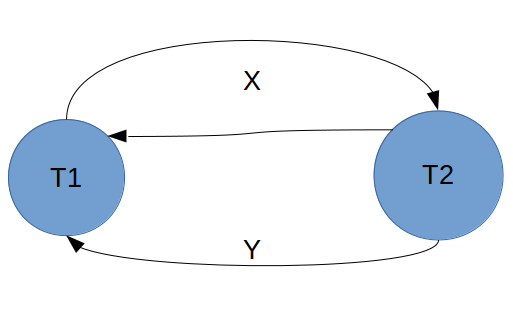
\includegraphics[scale=0.7]{41}
    \end{center}
    there is circle, so it is not schedule serialisable
    \item draw a table\\
    \begin{tabular}{ | c | c | c |c | c | c |c | c | c |}
        \hline
        T1 &      &      &      & W(Y) &      &      &      & R(X)\\
        \hline
        T2 &      &      &      &      & R(Y) &      & W(X) &     \\
        \hline
        T3 & R(X) &      &      &      &      & R(D) &      &     \\
        \hline
        T4 &      & W(Y) & W(Z) &      &      &      &      &     \\
        \hline
    \end{tabular}
    \begin{center}
        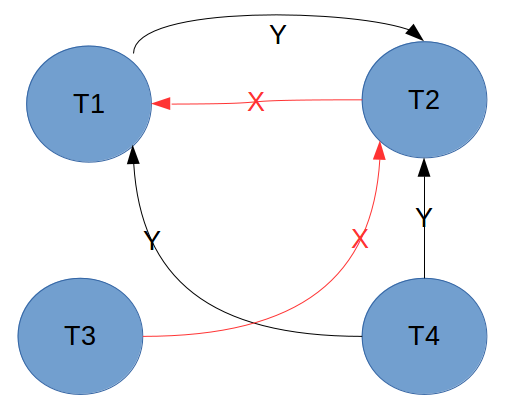
\includegraphics[scale=0.7]{42}
    \end{center}
    there is no circle, so it is schedule serialisable
\end{enumerate}

\end{document}